%     /home/jsbien/fc-search-codepoint
% Janusz S. Bień
% jsbien@uw.edu.pl

\documentclass[withmarginpar]{mwart}
\usepackage{fontspec}
\usepackage{polyglossia}
\usepackage{etoolbox}
\setmainlanguage{polish}
\setotherlanguage{english}
\usepackage{csquotes}
\usepackage{wrapfig}
%\usepackage{ccicons}
\usepackage[style=authoryear,backend=biber,backref=true,urldate=short]{biblatex}
%\addbibresource{jsbqed.bib}
\addbibresource{eab.bib}
\DefineBibliographyStrings{polish}{%
  byeditor = {red.},
  urlseen = {dostęp},
}

% http://tex.stackexchange.com/questions/166337/quotation-mark-quotation-sign-xelatex-polyglossia-csquotes
\DeclareQuoteStyle{polish}% I looked it up on Wikipedia, no idea if it's right
  {\quotedblbase}
  {\textquotedblright}
  [0.05em]
  {\textquoteleft}
  {\textquoteright}

% psuje tytuły???:
%  \usepackage{ulem}
\usepackage{metalogo}
\usepackage[polish]{varioref}

\def\eob{ę}
% DejaVuSans
% DejaVuSerif
%\setmainfont[Mapping=tex-text]{TeX Gyre Termes}
%\setmainfont[Mapping=tex-text]{DejaVuSerif}
% \char"EC10 \char"EC11 oraz \char"EC12
\def\orogate{\char"EC12}
\usepackage{relsize}

\usepackage{hyperref}

\usepackage{graphicx}
% [hyphens]: options clash
\usepackage{url}
%\usepackage{natbib}
\newcommand{\uname}[1]{{\relsize{-1}\texttt{#1}}}
\newcommand{\ucode}[1]{\texttt{#1}}
\newcommand{\mname}[1]{\texttt{#1}}
\newcommand{\mcode}[1]{\texttt{#1}}
\newcommand{\aname}[1]{\texttt{#1}}
\newcommand{\acode}[1]{\texttt{#1}}
\newcommand{\prname}[1]{\textsf{#1}}
%


\usepackage{draftwatermark}
\usepackage[doublespacing]{setspace}
\usepackage[draft]{fixme}

\usepackage[type={CC},modifier={by-sa}, version={3.0}]{doclicense}

\usepackage{appendix}
\renewcommand{\appendixpagename}{Dodatek}

\begin{document}
% ???:
%\gappto\captionslingua{\renewcommand{\chaptername}{Caput}}
%\gappto\captionspolish{\renewcommand{\figurename}{Ilustracja}}
\renewcommand{\figurename}{Ilustracja}

\title{Dokumenty DjVu w Internecie.\\ Reaktywacja}

\author{Janusz S. Bień}


\date{24 listopada 2020\\\doclicenseLongName}

\maketitle

\section{Wstęp}{}

Kilkanaście lat temu format DjVu był powszechnie używany m.in. w polskich
bibliotekach cyfrowych, gdzie około 80 \% publikacji było
udostępnianych właśnie w tym formacie \autocite[s. 311]{bc165}. Wsparcie dla tego
formatu było dostępne w praktycznie wszystkich przeglądarkach WWW dzięki
 odpowiedniej wtyczce.

% 37 bibliotek FBC (stan na dzień 17.04.2009

% Jak pokazują statystyki polskiej Federacji Bibliotek Cyfrowych (http://fbc.pionier.net.pl/
% owoc/attr-stats), ponad 80% publikacji w 37 bibliotekach (stan na dzień 17 kwietnia 2009
% r.) jest zapisanych w formacie DjVu.

% s. 311
% Dygitalizacja i komputeryzacja słowników
% na przykładzie „Słownika polszczyzny XVI wieku”

 Oprogramowanie do obsługi korpusów z wizualizacją trafień na skanach
 publikacji w formacie DjVu (nazywane \textsf{Poliqarp for DjVu} lub
 \textsf{Poliqarp/marasca}) wdrożone do eksploatacji w grudniu 2009
 r. i obecnie obsługujące witrynę
 \url{https://szukajwslownikach.uw.edu.pl}, zostało zaprojektowane
 przy założeniu, że użytkownik dysponuje w swojej przeglądarce WWW
 obsługą tego formatu (por. np. \cite{bc322}).

% Narzędzia dygitalizacji tekstów na potrzeby badań filologicznych

% https://www.researchgate.net/publication/336103761
% Skanowane teksty jako korpusy

Wtyczki do przeglądarek okazały się podatne na ataki i zostały
całkowicie wycofane z użytku. Zostały zastąpione przez
tzw. rozszerzenia, które ze względów bezpieczeństwa mają ograniczone
możliwości. Dostęp online do dokumentów DjVu stał się możliwy tylko za
pomocą ubogich --- żeby nie powiedzieć prymitywnych --- konwerterów na
aktualnie obsługiwane formaty. Nie spełniały one wymogów
\textsf{Poliqarp for DjVu}.

Rozwiązanie problemu pojawiło się około 4 lata temu, ale nie zostało
zauważone przez użytkowników DjVu. W październiku 2020 r. moją uwagę
na nie zwrócił Joachim Aleszkiewicz, za co serdecznie dziękuję.

Rozwiązanie to ma postać rozszerzenia --- dla Firefox, Chrome, Opera i
Edge\footnote{\url{https://github.com/andy-portmen/external-application-button/issues/55}}
--- o nazwie \textsf{External Application
  Button}\footnote{\url{https://github.com/andy-portmen/external-application-button}},
którego autorem jest Andy Portmen. Od wersji 0.4.0 z 25 października
2020 r. po odpowiednim skonfigurowaniu daje możliwości praktycznie
identyczne do oryginalnej
wtyczki\footnote{\url{https://github.com/andy-portmen/external-application-button/issues/50}}.

\section{Instalacja}
\label{sec:instalacja}


Cały proces instalacji i konfiguracji obsługi formatu DjVu obejmuje 4
etapy:

\begin{enumerate}
\item Instalacja \textsf{djview4}.
\item Instalacja roszerzenia EAB.
\item Konfiguracja rozszerzenia EAB.
\item Instalacja tzw. serwera lokalnego EAB.
\end{enumerate}

%\textbf{ad 1}

\subsection{djview4}
\label{sec:djview4}


W przypadku Linuksa instalacja \textsf{djview4} polega na instalacji
pakietu dostępnego w danej dystrybucji.

Dla MS Windows pobieramy i instalujemy
% \texttt{DjVuLibre-3.5.27_DjView-4.11_Qt5.15.1_Setup.exe} (lub nowsze)
dostępne pod adresem
\url{https://sourceforge.net/projects/djvu/files/DjVuLibre_Windows/3.5.27\%2B4.11/}

Dla 64-bitowej wersji MS Windows można też pobrać plik \texttt{djview.exe} ze strony
\url{https://github.com/jsbien/djview4/releases/tag/v20.11.05}; jest
to gotowy do użytku program, który nie wymaga instalacji. Należy
zapamietać lokalizację pliku na dysku lokalnym, bo informacja ta
będzie potrzebna później.

% Dla 32-bitowej wersji MS Windows należy zainstalować program z
% oficjalnej dystrybucji w sposób opisany w dodatku.

\subsection{Instalacja rozszerzenia}
\label{sec:inst-rozsz}


Rozszerzenie instalujemy standardowo, dalej omówimy ten proces na
przykładzie Firefoxa. Rozszerzenie można wyszukać po nazwie, można
też wejść na odpowiednią stronę:
\begin{itemize}
\item 
  Firefox; \url{https://addons.mozilla.org/en-US/pl/addon/external-application/}, por. il. \vref{fig:add-ons},
\item Chrome: \url{https://chrome.google.com/webstore/detail/external-application-butt/bifmfjgpgndemajpeeoiopbeilbaifdo},
\item Opera: \url{https://addons.opera.com/en/extensions/details/external-application-button/}
\item Edge: \url{https://microsoftedge.microsoft.com/addons/detail/external-application-butt/icfhhpfimihpdgglmdlnmpaadfeaacbk}
\end{itemize}

Po klinieciu \texttt{Dodaj do Firefoxa} zostaniemy poproszeni o
potwierdzenie, por. il. \vref{fig:first_perm}

\begin{figure}[h]
\centering
  
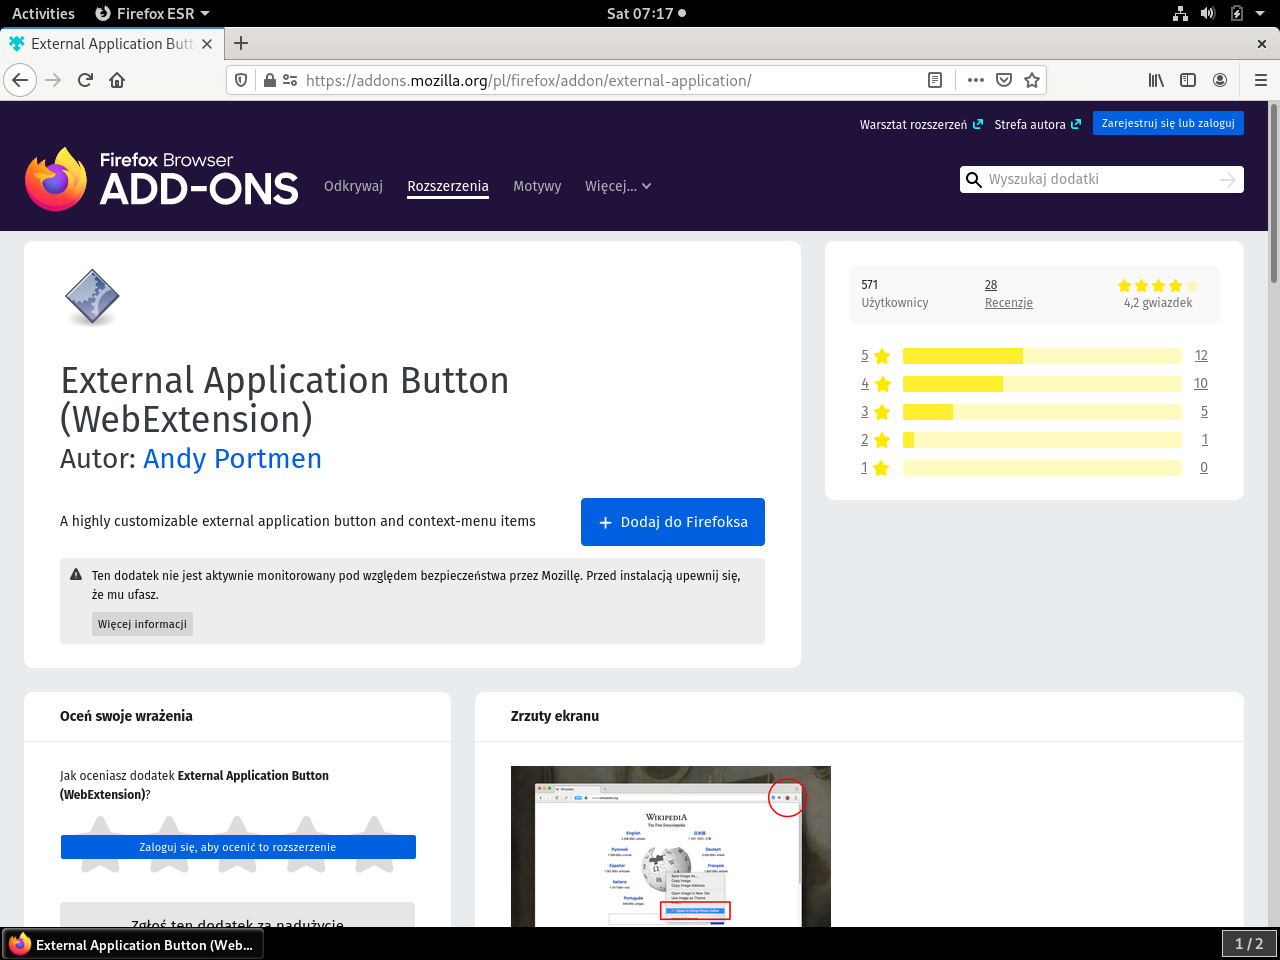
\includegraphics[width=0.95\hsize]{img/add-ons}

\caption{Strona rozszerzenia (Firefox)}
\label{fig:add-ons}
\end{figure}

\begin{figure}[h]
\centering
  
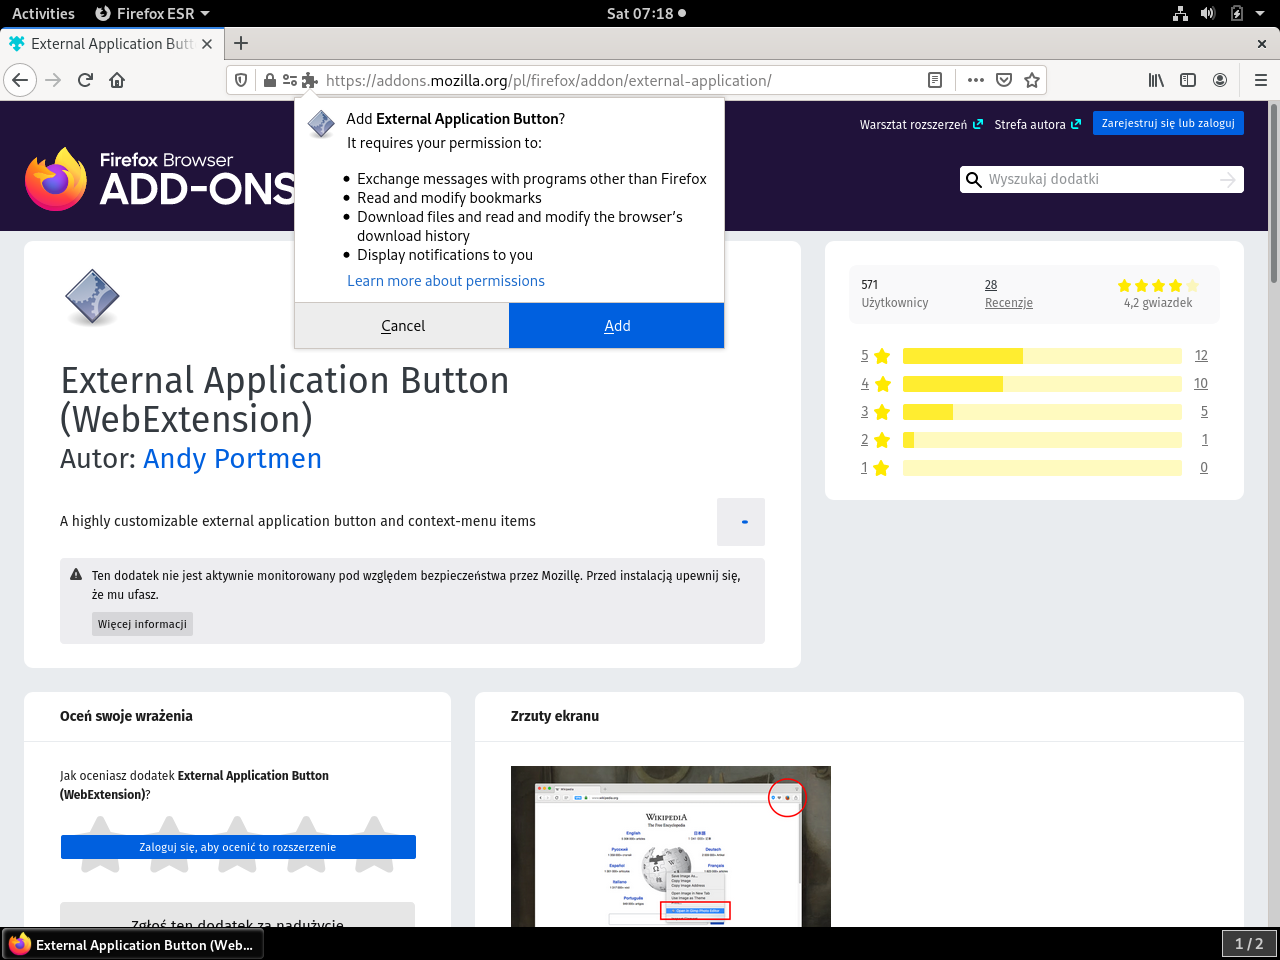
\includegraphics[width=0.95\hsize]{img/first_permissions}

\caption{Potwierdzenie instalacji i pierwsza zgoda na uprawnienia (Firefox)}
\label{fig:first_perm}
\end{figure}

\begin{figure}[h]
\centering
  
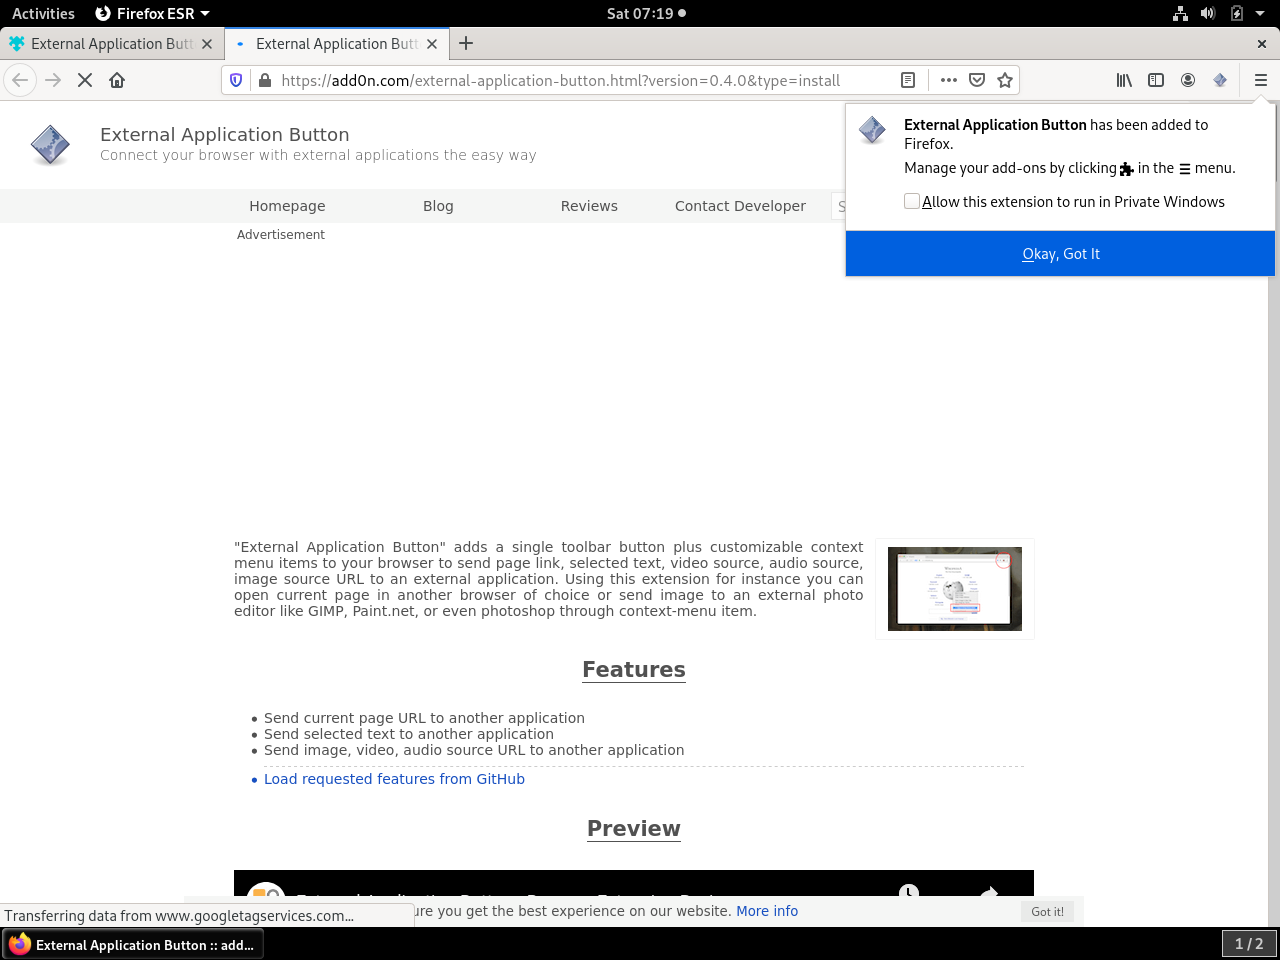
\includegraphics[width=0.95\hsize]{img/added}

\caption{Potwierdzenie zainstalowania (Firefox)}
\label{fig:added}
\end{figure}

Zainstalowanie zostanie potwierdzone komunikatem w okienku --- por
il. \vref{fig:added}. Jednocześnie zostaje wyświetlona strona z
różnymi informacjami na temat rozszerzenia, a w prawym górnym rogu
przeglądarki pojawi się ikona rozszerzenia.

%\newpage
%\clearpage
%\textbf{ad 3}

\subsection{Konfiguracja rozszerzenia}
\label{sec:konf-rozsz}


Instrukcję konfiguracji sformułował Joachim Aleszkiewicz, ja ją tylko
nieznacznie uzupełniłem.

Do konfiguracji przechodzimy klikając na wspomnianą wyżej ikonę
rozszerzenia, co powoduje wyświetlenie formularza ---
por. il. \vref{fig:conf}.

\begin{figure}[h]
\centering
  
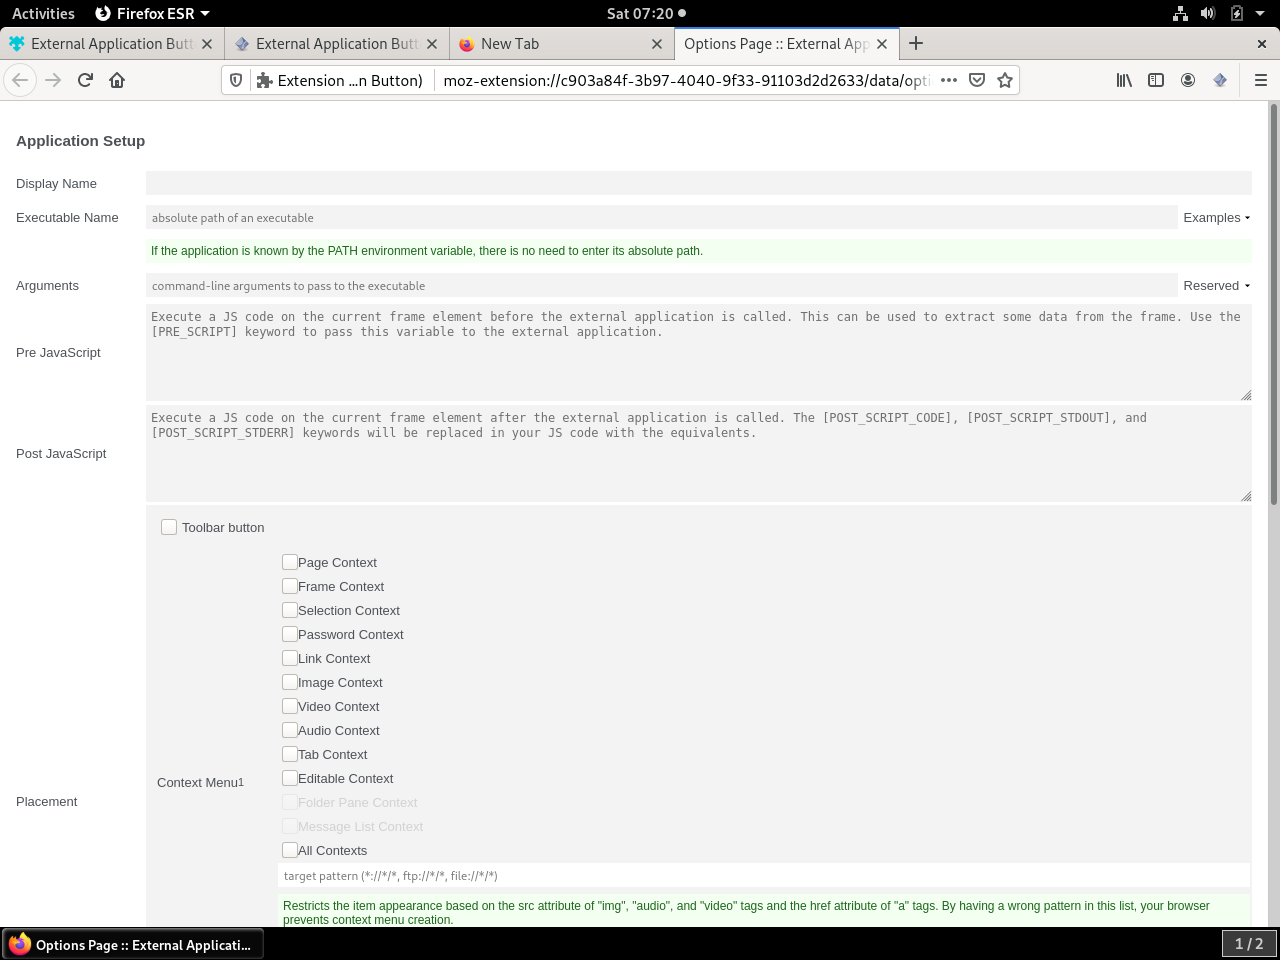
\includegraphics[width=0.95\hsize]{img/setup}

\caption{Konfiguracja (Firefox)}
\label{fig:conf}
\end{figure}

W trakcie wypełniania pojawi się kolejne pytanie o uprawnienia ---
patrz il. \vref{fig:sec_per}.

\begin{figure}[h]
\centering
  
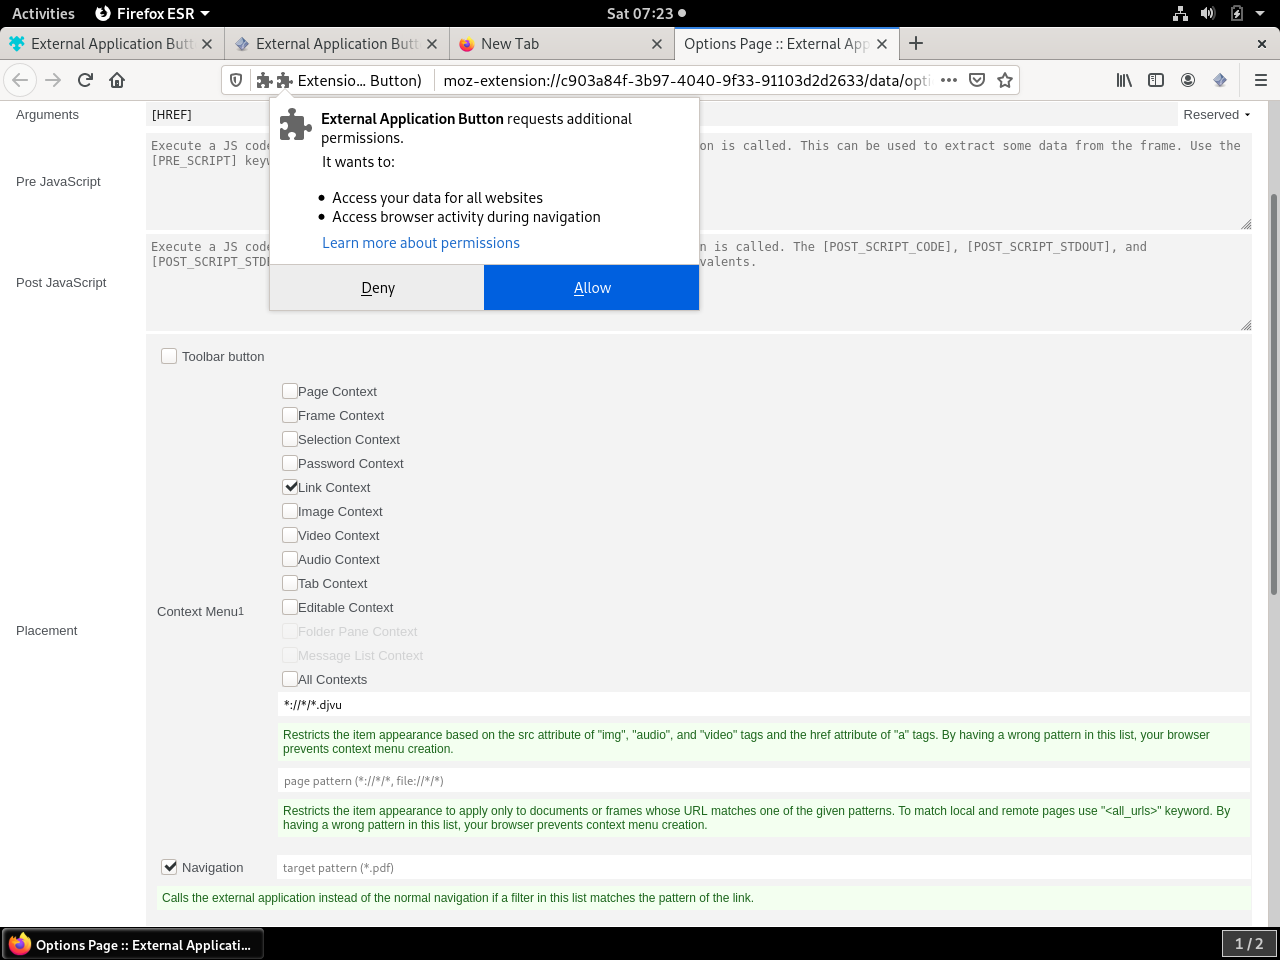
\includegraphics[width=0.95\hsize]{img/second_permissions}

\caption{Konfiguracja --- pytanie o uprawnienia (Firefox)}
\label{fig:sec_per}
\end{figure}

Wypełniamy tylko następujące pola:
\begin{enumerate}
\item \texttt{Display Name}: \texttt{DjView} (lub inna nazwa wskazująca na przeznaczenie);
\item \texttt{Executable name}:
  \begin{itemize}
  \item \texttt{djview} (Linux),
  \item \verb|c:\Program Files(x86)\DjVuLibre\djview.exe| (MS Windows,
    również w wersjach językowych innych niż angielski --- należy
    zwrócić uwagę na spacje i kasztę liter);
  \end{itemize}
\item \texttt{Arguments}: \texttt{[HREF]};
\item Sekcja \texttt{Toolbar button}: zaznaczamy tylko \texttt{Link Context};
\item Sekcja \texttt{Context menu}, pole \texttt{Target Pattern}: \texttt{*://*/*.djvu*};
\item Sekcja \texttt{Navigation}: zaznaczamy i wpisujemy \texttt{*.djvu*}
\end{enumerate}

Następnie klikamy na \texttt{Add Application} --- por
il. \vref{fig:add_but}.  W polu \texttt{List of applications} pojawia
się \texttt{DjView}, a \texttt{Add Application} zmienia się na
\texttt{Update Application}.

\begin{figure}[h]
\centering
  
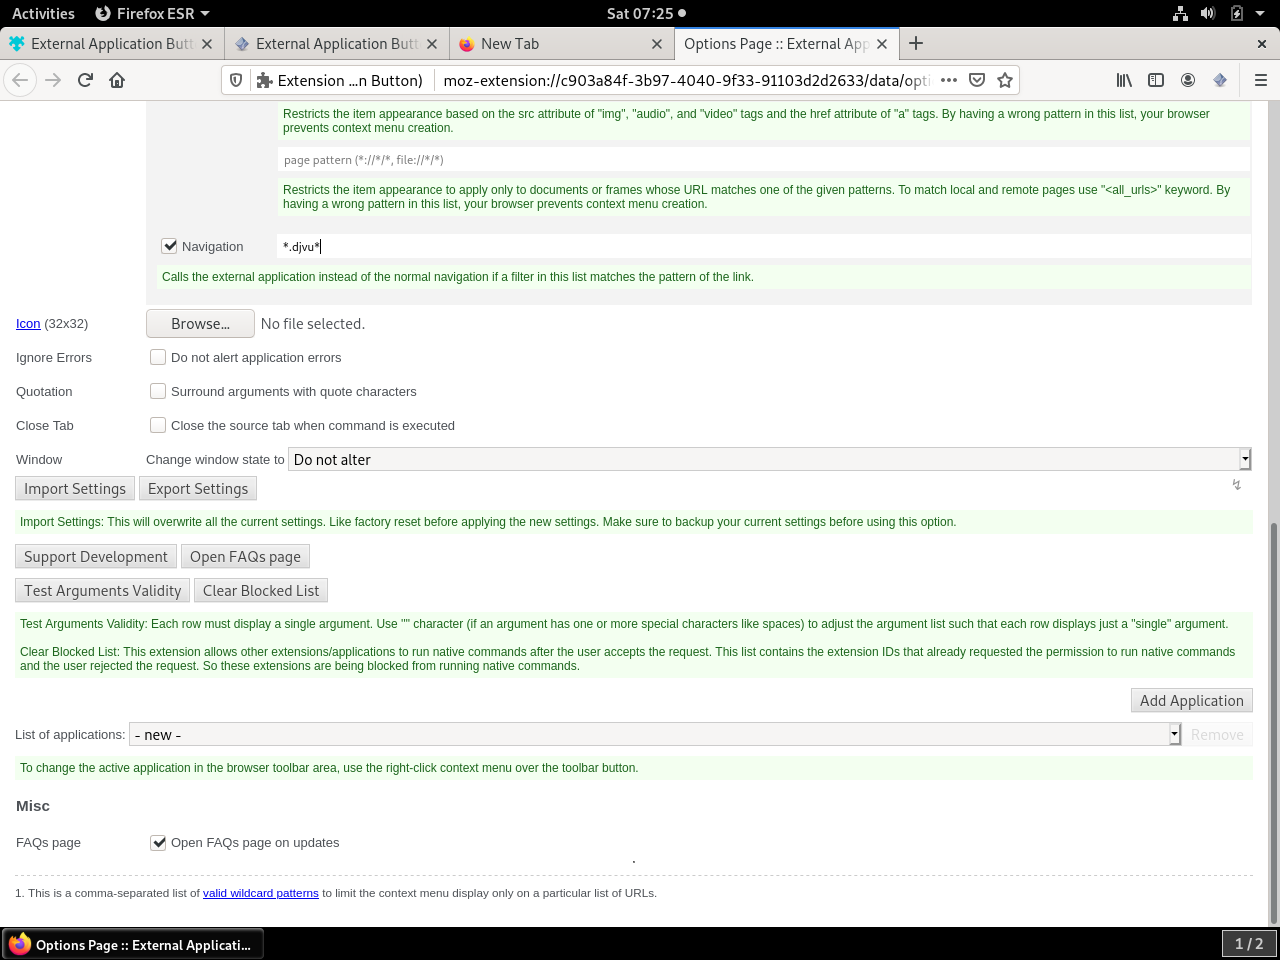
\includegraphics[width=0.95\hsize]{img/add_button}

\caption{Zapisywanie konfiguracji (Firefox)}
\label{fig:add_but}
\end{figure}



\clearpage

%\textbf{ad 4}

\subsection{Instalacja lokalnego serwera}
\label{sec:inst-lokaln-serw}

\subsubsection{Własciwa instalacja}
\label{sec:wasciwa-instalacja}


Instalację lokalnego serwera (czasami nazywanego przez autora lokalnym
klientem) rozpoczynamy od próby otwarcia jakiegoś dokumentu DjVu,
np. wspomnianego wcześniej
\url{https://djvu.szukajwslownikach.uw.edu.pl/IMPACT_GT_1/00426979.djvu}. Zostaniemy
przekierowani do strony \texttt{One Last Step} --- patrz
il. \vref{fig:last_step}. Na stronie znajdują się trzy polecenia:
\begin{enumerate}
\item Pierwsze z nich to \texttt{Click here to download the
    package for your OS}, należy kliknąć na \texttt{here}.
 \item Drugie polecenie to rozpakowanie pobranego archiwum.
 \item Trzecie polecenie to właściwa instalacja --- wykonanie
   \texttt{./install.sh} (w katalogu, do którego został rozpakowany) w
   przypadku Linuksa i dwukrotne kliknięcie na \texttt{install.bat} w
   przypadku MS Windows.
%   --- wbrew instrukcji nie musi to być katalog
%   administratora\footnote{https://github.com/andy-portmen/external-application-button/issues/54}).
\end{enumerate}

\subsubsection{Test instalacji}
\label{sec:test-instalacji}

\begin{figure}[h]
\centering
  
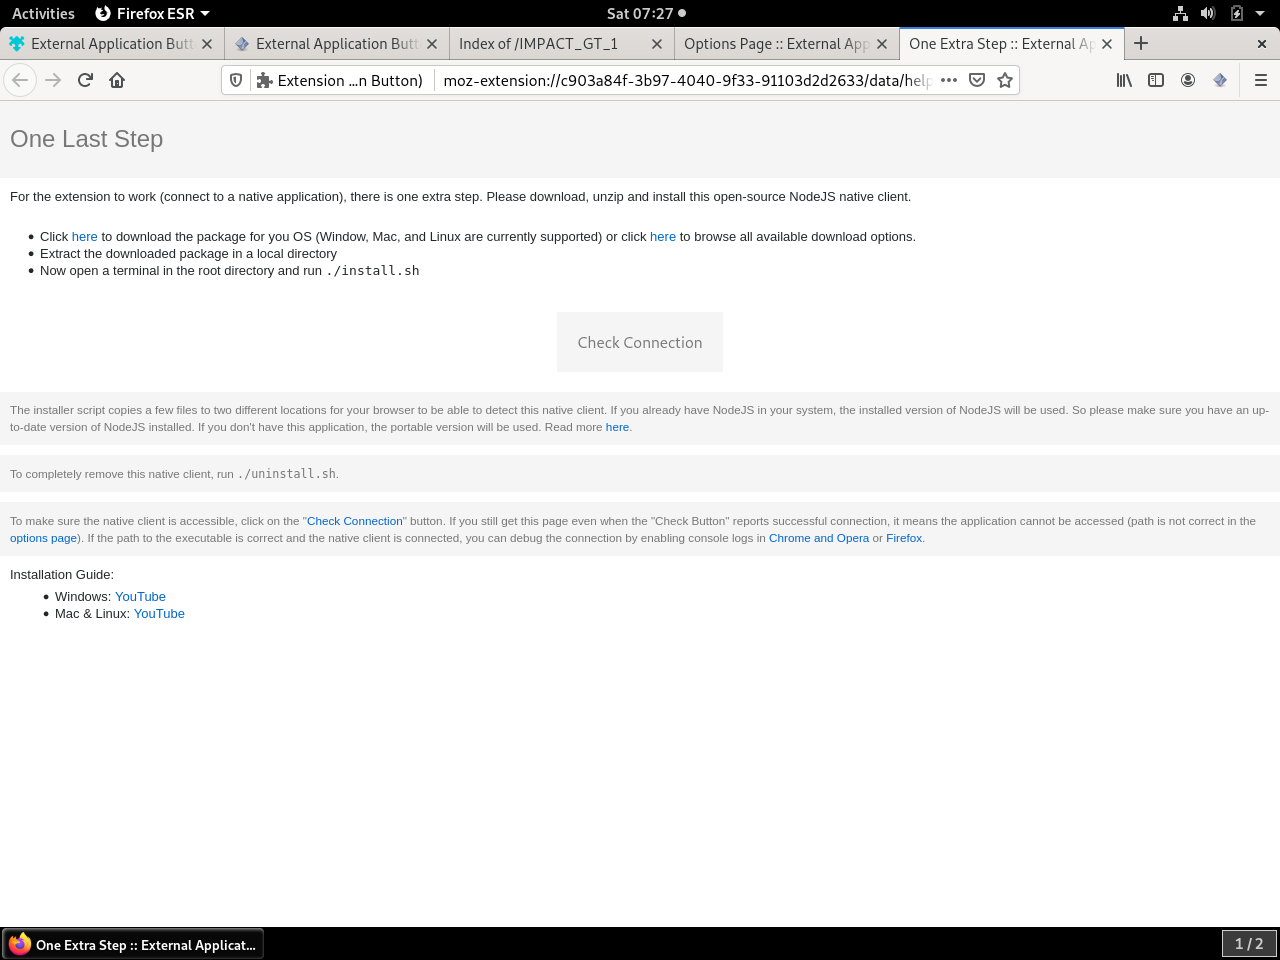
\includegraphics[width=0.95\hsize]{img/last_step}

\caption{Instalacja lokalnego serwera (Firefox)}
\label{fig:last_step}
\end{figure}

\begin{figure}[h]
\centering
  
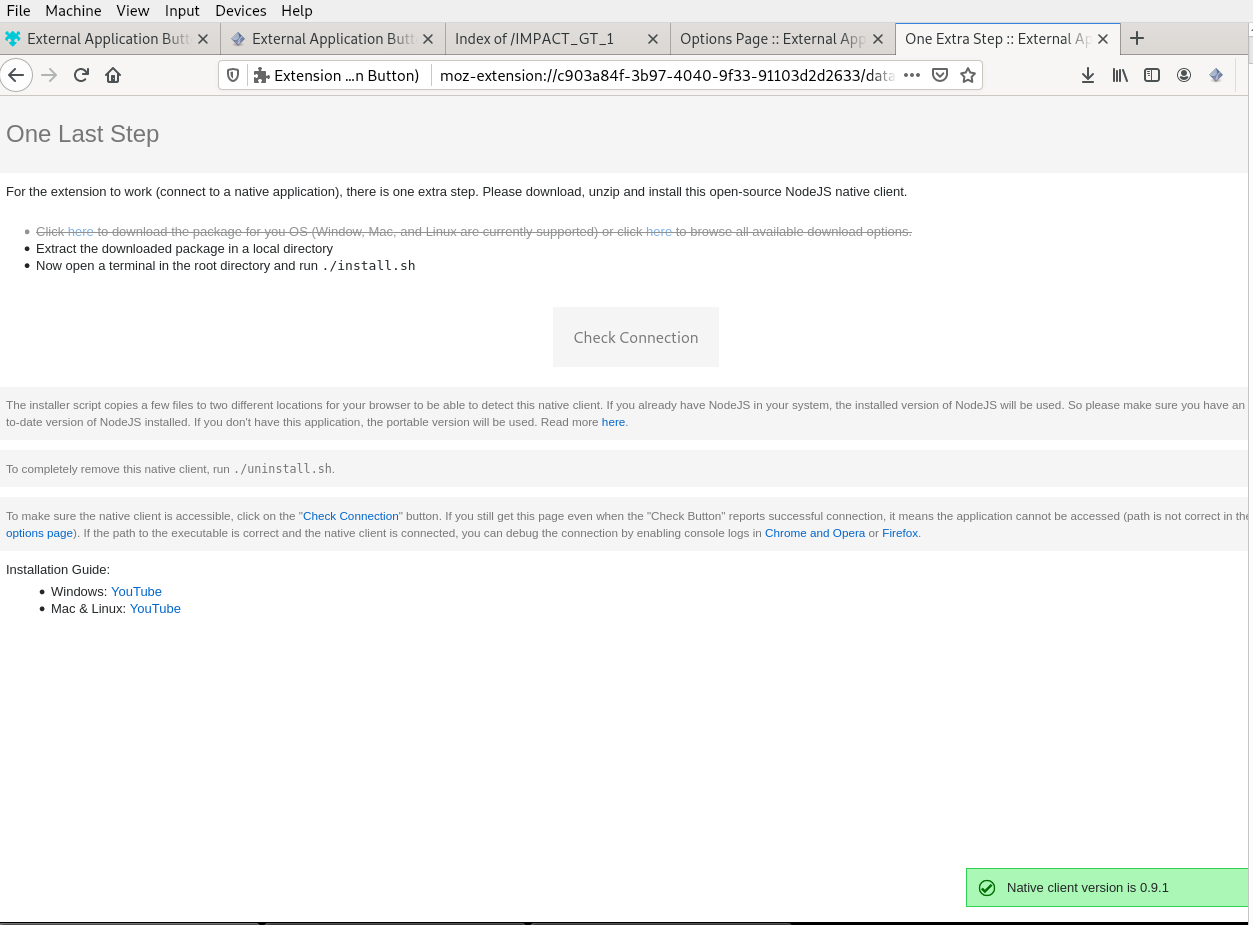
\includegraphics[width=0.95\hsize]{img/client}

\caption{Weryfikacja lokalnego serwera}
\label{fig:client}
\end{figure}

\textbf{Instalacja i konfiguracja jest zakończona --- kliknięcie na
  link do dokumentu DjVu spowoduje teraz jego otworzenie w specjalnie
  uruchomionej przegladarce \textsf{djview}.}


Poprawność instalacji sprawdzamy klikając na \texttt{Check Connection}
--- powinniśmy otrzymać potwierdzenie takie, jak na
il. \vref{fig:client}.

\clearpage

\subsection{Ewentualne problemy}
\label{sec:ewentualne-problemy}


W razie problemów z instalacją rozszerzenia możemy skorzystać z
instrukcji w postaci trzyminutowych filmów:
\begin{itemize}
\item Linux: \url{https://www.youtube.com/watch?v=bB4Bj_APg4g},
\item Windows: \url{https://www.youtube.com/watch?v=18jAqTXBiZA}.
\end{itemize}

Jeśli plik DjVu się nie otwiera, lecz zamiast tego następuje
przekierowanie na stronę z komunikatem o błędzie ---
por. il. \vref{fig:2debug} --- wówczas zgodnie z instrukcją należy
najpierw sprawdzić połączenie z lokalnym serwerem, a jeśli jest
poprawne, przejrzeć log konsoli przeglądarki. W Firefoxie najprościej
włączyć konsolę skrótem klawiaturowym \texttt{Ctrl+Shift+J}.

\begin{figure}[h]
\centering
  
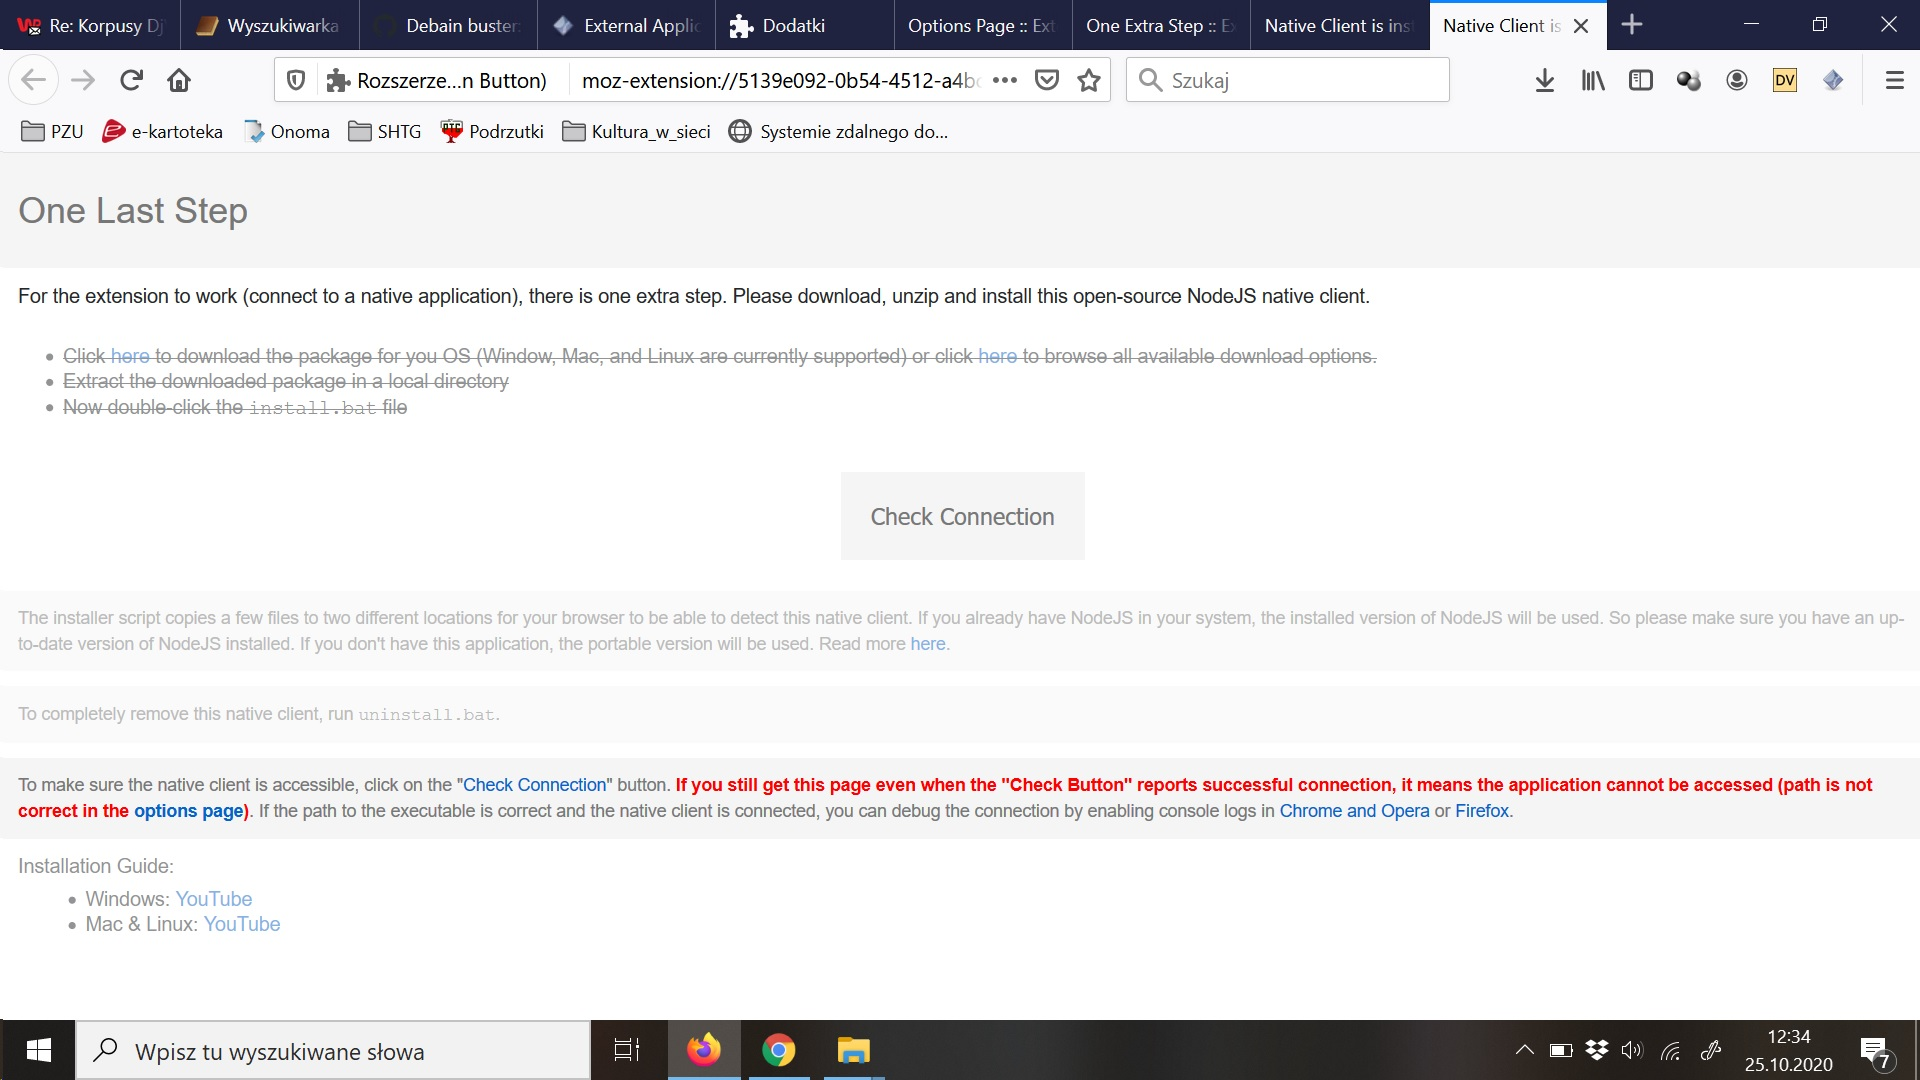
\includegraphics[width=0.95\hsize]{img/2debug}

\caption{Komunikat o błędzie}
\label{fig:2debug}
\end{figure}

\section{Zastosowania}
\label{sec:zastosowania}



%\textbf{Zastosowania}

\begin{figure}[h]
\centering
  
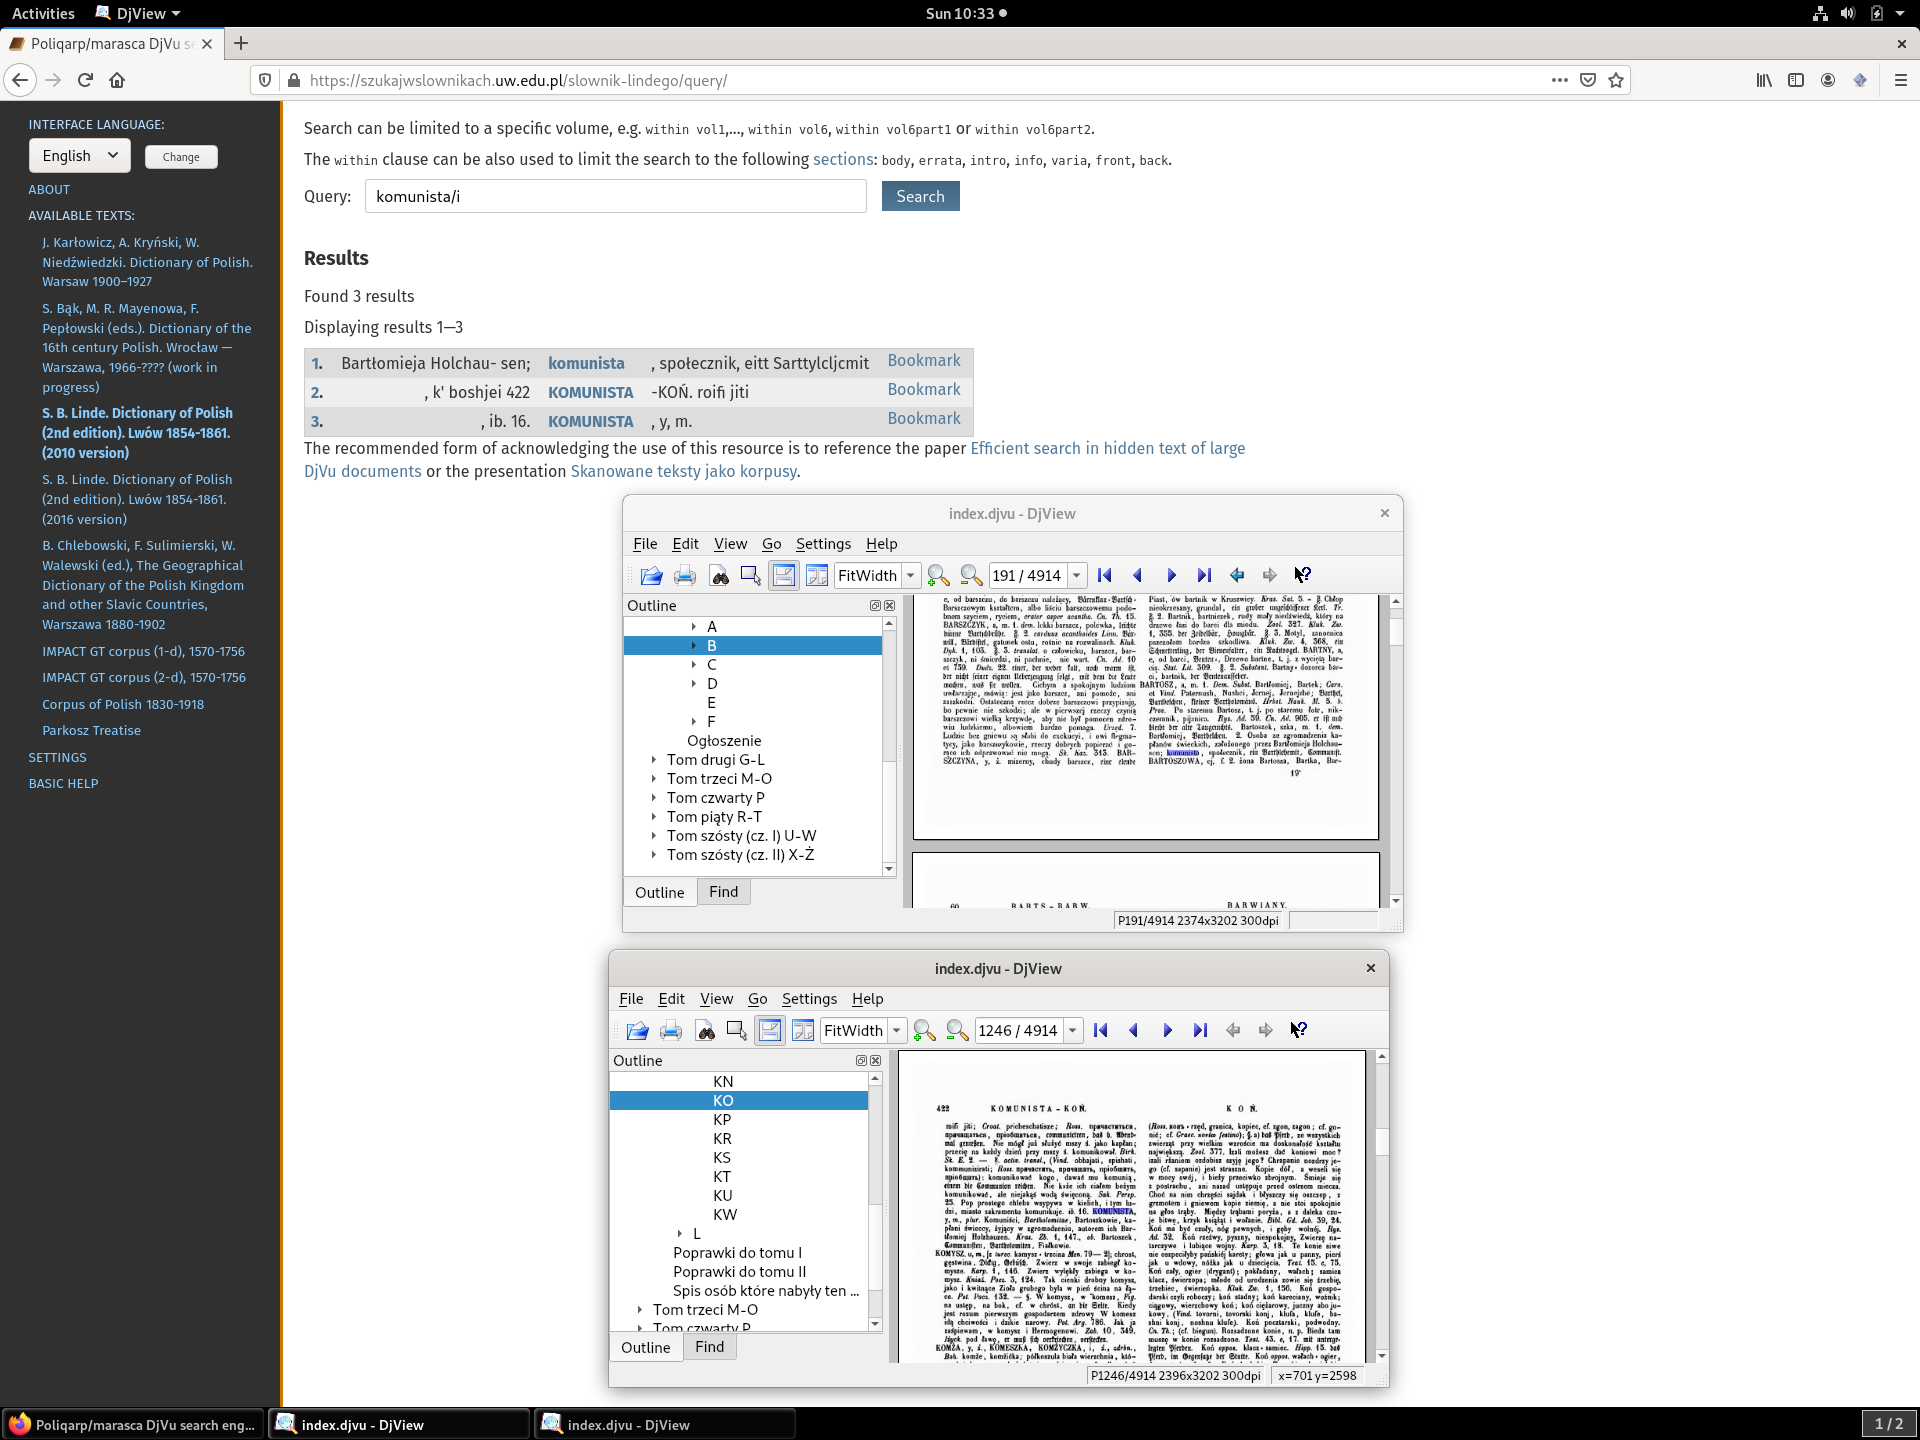
\includegraphics[width=0.95\hsize]{img/poliqarpfordjvu}

\caption{\textsf{Poliqarp for DjVu}}
\label{fig:poliqarp4djvu}
\end{figure}


Zainstalowaną obsługę formatu DjVu możemy wykorzystywać teraz na
potrzeby wspomnianej witryny \url{https://szukajwslownikach.uw.edu.pl}
--- patrz il. \vref{fig:poliqarp4djvu}, ale możemy stosować ją również
do wygodnego przeglądania dokumentów w bibliotekach
cyfrowych. Rozważmy dla przykładu pierwszy tom pierwszego wydania
słownika Lindego w Kujawsko-Pomorskiej Bibliotece
Cyfrowej\footnote{\url{https://kpbc.umk.pl/publication/8176}}. Jeśli
zamierzamy korzystać z niego systematycznie, najlepiej pobrać całość i
przeglądać lokalnie za pomocą djview. Jeśli korzystamy tylko
okazjonalnie, klikamy na \texttt{Pokaż treść}. Otworzą nam się dwa
panele: po prawej wyświetli sie pierwsza strona w domyślnym widoku, po
lewej mamy dwie zakładki: \textit{Metadane} i \textit{Lista
  plików}. Wybieramy \textit{Lista plików} i odszukujemy plik
indeksowy --- ma on nazwę krótszą niż pliki zawierające poszczególne
strony\footnote{%Jest to konkretnie
\url{https://kpbc.umk.pl/Content/12850/DjVu/Filologia_001_01_Tom_01.djvu}}. Po
klinięciu na plik cały dokument otwiera się w \textsf{djview} i możemy
porównać, który sposób wyświetlania jest dla nas wygodniejszy.

Na zakończenie warto przypomnieć, że dla użytkowników witryny
\url{https://szukajwslownikach.uw.edu.pl} nadal zalecany jest program
\textsf{djview4poliqarp}\footnote{\url{htps://bitbucket.org/mrudolf/djview-poliqarp/downloads/}}
--- por. np. \cite{bien_elektroniczne_2018}; wersja dla MS Windows nie
wymaga instalacji. Okresowo korzystanie z programu było utrudnione lub
nawet niemożliwe (m.in ze względu na różne zmiany na serwerze
niezbędne ze względów bezpieczeństwa), ale wersja z lipca 2020
r. wydaje się działać całkowicie poprawnie --- patrz
il. \vref{fig:djview4poliqarp}.


\begin{figure}[h]
\centering
  
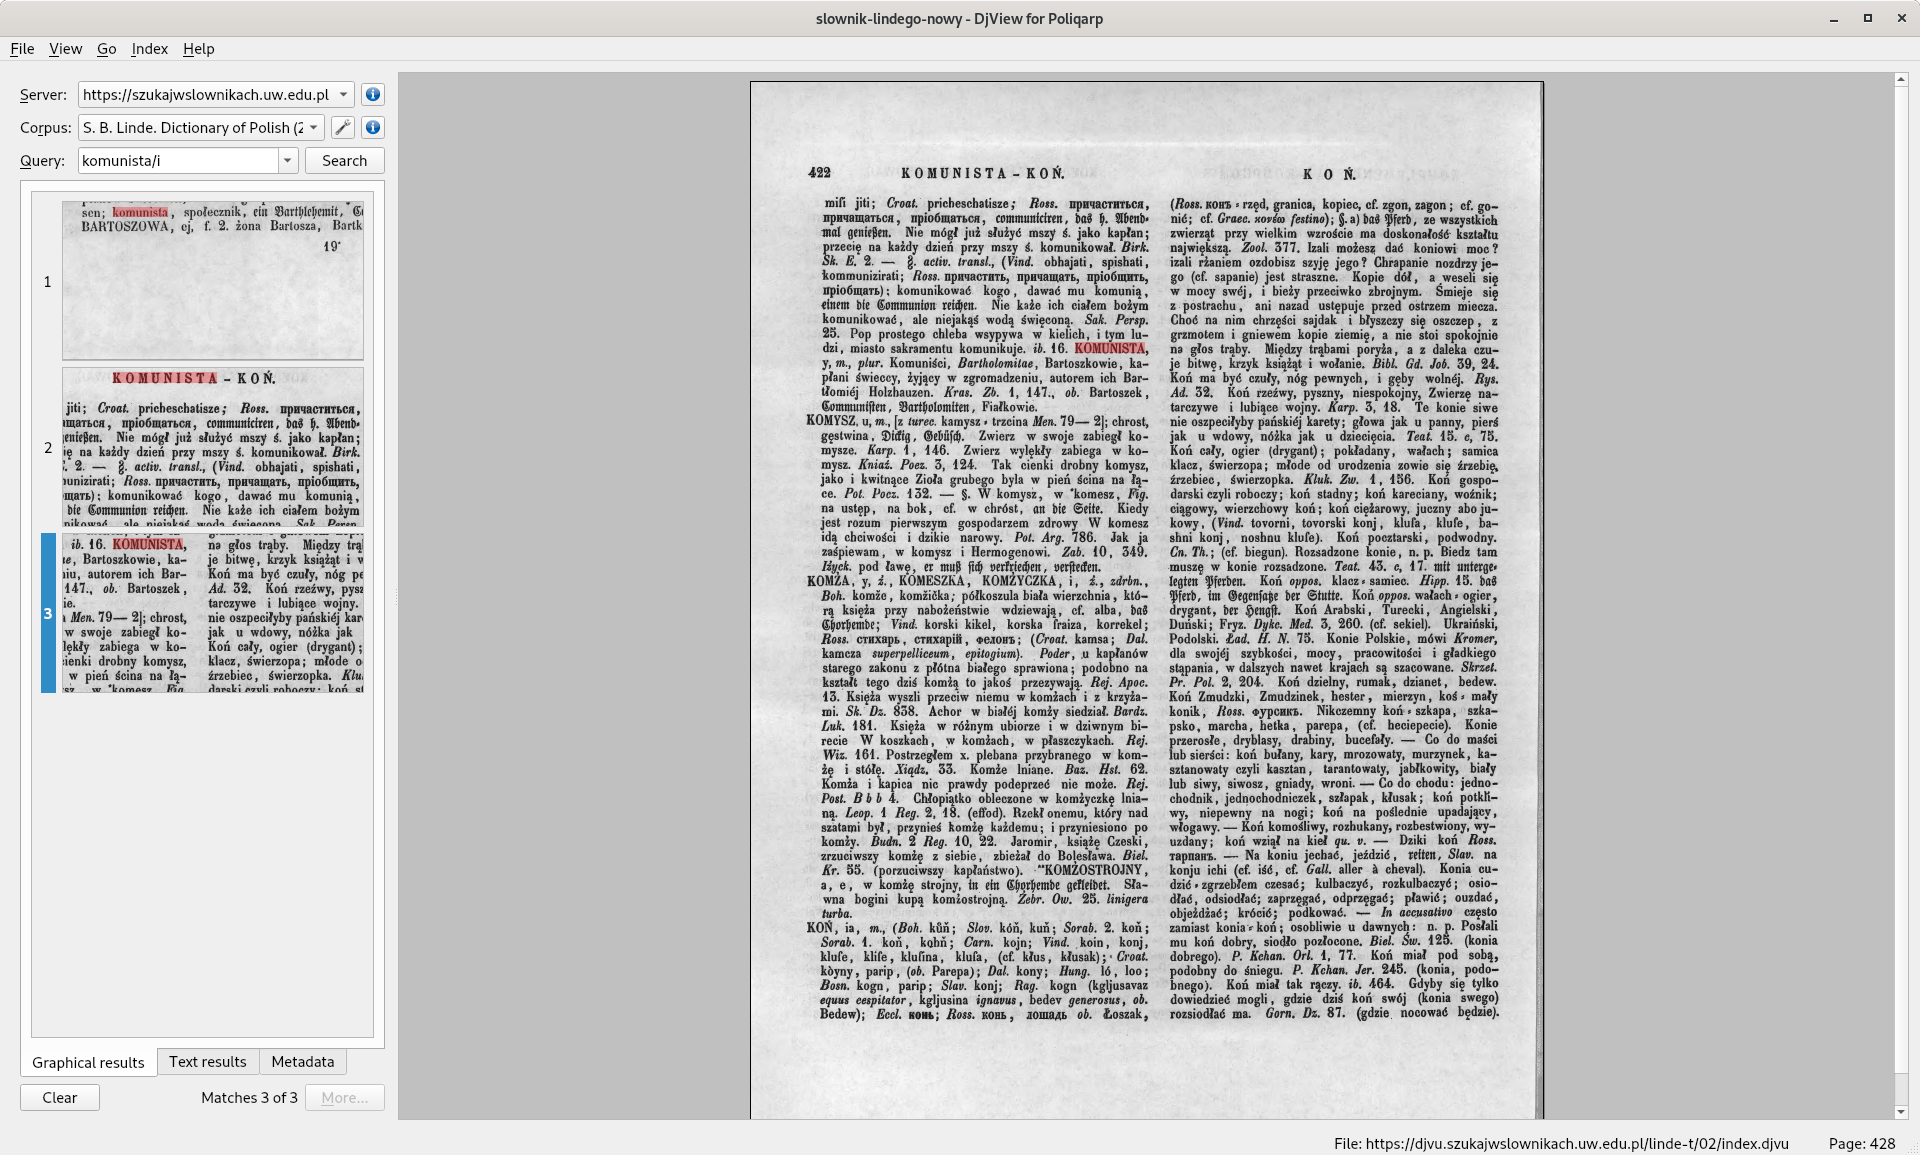
\includegraphics[width=0.95\hsize]{img/djview4poliqarp}

\caption{\textsf{djview4poliqarp}}
\label{fig:djview4poliqarp}
\end{figure}

%Alexander Trufanov djview4shapes

% Biblioteki cyfrowe zareagowały na to udostępnianiem ubogich
% przeglądarek zastepczych, pozbawionych wielu funkcjkonwertowaniem dokumentów DjVu ``w locie'' na
% HTML lub całkowitym

% Język Polski. 2000, nr 1/2 (styczeń/kwiecień)
% http://mbc.malopolska.pl/publication/35488 HTML5

% content presentation
% http://mbc.malopolska.pl/dlibra/list?mimetype=image/x.djvu&sec=false&content_url=/Content/32812/index.djvu

% http://mbc.malopolska.pl/dlibra/Content/32812/index.djvu


% Let My browser handle publication's content.
% DjVU - HTML5
% DjVu built-in applet
% DjVu browser plug-in required

% 1. pobiera indeks
% 2
% 3. java
% Język Polski i Poradnik Językowy. R. 3 (1916) = z. 1-10


\printbibliography
% \appendix
% \appendixpage
% \section{Instalacja djview z oficjalnej dystrybucji (nierekomendowana)}
% \label{sec:instalacja-djview-z}


% \subsection{Właściwa instalacja}
% \label{sec:waciwa-instalacja}
%   Instalacja właściwego programu polega na pobraniu instalatora ze
%   strony \url{http://djvu.sourceforge.net/djview4.html}.
%   % \item

% \subsection{Test OpenSSL}
% \label{sec:test-openssl}
% Test OpenSSL polega na próbie otworzenia za pomocą \texttt{File ---
%   Open Location} np. dokumentu
% \url{https://djvu.szukajwslownikach.uw.edu.pl/IMPACT_GT_1/00426979.djvu};
% jesli pojawi się błąd \texttt{TLS initialization failed}, to znaczy,
% że potrzebna jest dodatkowo instalacja bibliotek \textsf{OpenSSL}
% (por. \url{https://sourceforge.net/p/djvu/bugs/321/}). Niestety nie
% może być to po prostu najnowsza wersja tych bibliotek, lecz wersja
% zgodna z wersją \textsf{djview}. Dka aktualnie najnowszej wersji
% \textsf{djview}, tj.
%   \begin{quote}
% \verb|DjVuLibre-3.5.27_DjView-4.11_qt5_beta1_Setup.exe|,
% \end{quote}
% potrzebne jest \textsf{OpenSSL} w wersji 1.1.1g.

% Instalacja jest opisana w następnych punktach. Nawet bez instalacji
% OpenSSL \textit{djview} może być uzywana do przegladania dokumentów
% pobranych na dysk lokalny.
% % \item

% \subsection{Pobranie właściwej wersji OpenSSL i dołączenie do djview4}
% \label{sec:pobr-wasc-wersji}
%  Ze strony
%   % \url{https://slproweb.com/products/Win32OpenSSL.html}
%   \url{https://bintray.com/vszakats/generic/openssl/1.1.1g} (adres
%   wskazał mi pośrednio Joachim Aleszkiewicz) należy pobrać archiwum
%   \begin{quote}
% \texttt{
%     openssl-1.1.1g-win32-mingw.zip}
% \end{quote}
% i rozpakowanie go.  Następnie
%   należy skopiować \verb|libcrypto-1_1.dll| i \verb|libssl-1_1.dll|
%   % z katalogu \verb|c:\Program Files (x64)\OpenSSL-Win32|
%   do katalogu \verb|c:\Program Files(x86)\DjVuLibre\|, gdzie znajduje
%   się plik \texttt{djview.exe} (wymagane uprawnienia
%   administratora). Następnie należy powtórzyć test (File --- Open Recent),
%   dokument powinien się teraz otworzyć.
% %\end{itemize}
% %\newpage
% %\textbf{ad 2}


\end{document}

        
%%% Local Variables: 
%%% coding: utf-8-unix
%%% mode: latex
%%% TeX-master: t
%%% TeX-PDF-mode: t
%%% TeX-engine: luatex
%%% End: 
